\documentclass{article}
\usepackage{amsmath}
\usepackage{amssymb}
\usepackage{fullpage}
\usepackage[parfill]{parskip}
\usepackage{graphicx}
\newcommand*{\horzbar}{\rule[.5ex]{2.5ex}{0.5pt}}
\newcommand{\pd}[2]{\frac{\partial #1}{\partial #2}}
\title{Assignment 1 writeup}
\author{Thomas Lu}
\date{}
\begin{document}
\maketitle
\section{Problem 1}
(a) We have
\begin{align*}
\text{softmax}(\mathbf{x} + c)_i &= \frac{e^{x_i + c}}{\sum_j e^{x_j + c}}\\
&= \frac{e^c(e^{x_i})}{e^c\sum_j e^{x_j}}\\
&= \frac{e^c}{e^c} \frac{e^{x_i}}{\sum_j e^{x_j}}\\
&= \frac{e^{x_i}}{\sum_je^{x_j}}\\
&= \text{softmax}(\mathbf{x})_i,
\end{align*}
so $\text{softmax}(\mathbf{x} + c) = \text{softmax}(\mathbf{x}),$ as desired.

\section{Problem 2}
(a) We have
\begin{align*}
\sigma(x) &= \frac{1}{1 + e^{-x}}\\
\sigma'(x) &= \frac{d}{dx} (1 + e^{-x})^{-1}\\
&=  -(1 + e^{-x})^{-2}\frac{d}{dx}\left(1 + e^{-x}\right) \\
&= -\left(\frac{1}{1 + e^{-x}}\right)^2 \left(-e^{-x}\right)\\
&= \left(\frac{1}{1 + e^{-x}}\right)\left(1 - \frac{1}{1 + e^{-x}}\right)\\
&= \left(\sigma(x)\right)\left(1 - \sigma(x)\right).
\end{align*}

(b) We have $\hat{y} = \text{softmax}(\theta).$ Suppose that $y$ is one-hot with $y_k = 1$. Then
\begin{align*}
\frac{\partial}{\partial \theta_j} CE(y, \hat{y}) &= \frac{\partial}{\partial \theta_j} \sum_i -y_i \log \frac{e^{\theta_i}}{\sum_i e^{\theta_i}}\\
&= -\frac{\partial}{\partial \theta_j} \log\frac{e^{\theta_k}}{\sum_i e^{\theta_i}}\\
&= \frac{\partial}{\partial \theta_j} \left(\log\left(\sum_i e^{\theta_i}\right) - \log e^{\theta_k} \right)\\.
\end{align*}
We now split into two cases. If $j \ne k$, then
\begin{align*}
\frac{\partial}{\partial \theta_j} CE(y, \hat{y}) &= \frac{\partial}{\partial \theta_j} \left(\log\left(\sum_i e^{\theta_i}\right) - \log e^{\theta_k} \right)\\
&= \frac{1}{\sum_i e^{\theta_i}}(e^{\theta_j})\\
&= \text{softmax}(\theta)_j.
\end{align*}
If $j = k$, then
\begin{align*}
\frac{\partial}{\partial \theta_j} CE(y, \hat{y}) &= \frac{\partial}{\partial \theta_k} \left(\log\left(\sum_i e^{\theta_i}\right) - \log e^{\theta_k} \right)\\
&= \frac{1}{\sum_i e^{\theta_i}}(e^{\theta_k}) - \frac{\partial}{\partial \theta_k}\theta_k\\
&= \text{softmax}(\theta)_k - 1.
\end{align*}
Thus
$$\vec{\nabla}_{\theta} CE(y, \hat{y}) = \text{softmax}(\theta) - y.$$

(c) We begin with a couple of theorems:

\textbf{Theorem:} If $f_1, f_2, \dots, f_n, g$ are differentiable, and
$$y = g(f_1(x), f_2(x), \dots, f_n(x)),$$
then
$$\frac{dy}{dx} = \sum_{i=1}^n \frac{\partial y}{\partial f_i} \frac{df_i}{dx}.$$

\textbf{Theorem:} If $x$ and $y$ are row vectors and $z$ is a scalar, and $f$ and $g$ are differentiable with $y = f(x)$ and $z = g(y)$, then
$$\frac{\partial z}{\partial x} = \frac{\partial z}{\partial y}\frac{\partial y}{\partial x},$$
where
$$\left(\frac{\partial y}{\partial x}\right)_{ij} = \frac{\partial y_i}{\partial x_j}.$$

We now compute $\partial J/\partial x$. Letting $z_1 = xW_1 + b_1$ and $z_2 = hW_2 + b_2$, we have
$$\frac{\partial J}{\partial x} = \frac{\partial J}{\partial z_2} \frac{\partial z_2}{\partial h} \frac{\partial h}{\partial z_1} \frac{\partial z_1}{\partial x}.$$
We evaluate the partials on the RHS of the above equation in sequence. We have:
\begin{align*}
\frac{\partial J}{\partial z_2} &= \text{softmax}(z_2) - y\\
\frac{\partial z_2}{\partial h} &= W_2^T\\
\frac{\partial h}{\partial z_1} &= \text{diag}(\sigma(z_1))\text{diag}(1 - \sigma(z_1))\\
\frac{\partial z_1}{\partial x} &= W_1^T\\
\Rightarrow \frac{\partial J}{\partial x} &= (\text{softmax}(z_2) - y)W_2^T\text{diag}(\sigma(z_1))\text{diag}(1 - \sigma(z_1))W_1^T\\
&= (\text{softmax}(z_2) - y) W_2^TW_1^T\circ \sigma(z_1) \circ (1 - \sigma(z_1))
\end{align*}
where $\text{diag}(v)$ denotes the diagonal matrix $D$ with $D_ii = v_i$ and 1 denotes a vector of ones where appropriate.

(d) There are four groups of parameters:
\begin{itemize}
\item $b_1$, a bias vector with $H$ entries,
\item $b_2$, a bias vector with $D_y$ entries,
\item $W_1$, a $D_x \times H$ weight matrix, and
\item $W_2$, a $H \times D_y$ weight matrix.
\end{itemize}
Thus the total number of parameters is
$$H + D_y + HD_x + HD_y = D_y(H + 1) + H(D_x + 1).$$

\section{Problem 3}
(a) Let $V$ be our vocabulary, and for $o, c \in V$, let $v_c$ denote the center word (column) vector for $c$ and $u_o$ denote the outer word (column) vector for $o$. Let $U$ denote the matrix
$$
\left[
\begin{array}{ccc}
\horzbar & u_{w_1}^T \horzbar \\
\horzbar & u_{w_2}^T \horzbar \\
& \vdots & \\
\horzbar & u_{w_N}^T \horzbar \\
\end{array}
\right],
$$
where $V = \{w_1, w_2, \dots, w_N\}$. Let 
$$\hat{y}_i = p(w_i | c) = \frac{\exp(u_{w_i}^Tv_c)}{\sum_{w \in V}\exp(u_w^Tv_c)}$$
and $\hat{y} = [\hat{y}_1, \hat{y}_2, \dots, \hat{y}_N].$ Supposing that $y$ is one-hot with the one at $o$, we have
\begin{align*}
\pd{J}{v_c} &= \pd{}{v_c} CE(y, \hat{y})\\
&= -\pd{}{v_c} \sum_{i=1}^N y_i \log \hat{y}_i \\
&= -\pd{}{v_c} \log \frac{\exp(u_o^Tv_c)}{\sum_{w\in V} \exp\left(u_w^Tv_c\right)}\\
&= -\pd{}{v_c} \left( \log\left(\exp(u_o^Tv_c)\right) - \log\left(\sum_{w\in V} \exp\left(u_w^Tv_c\right)\right)\right)\\
&= -u_o + \frac{1}{\sum_{w\in V}\exp( u_w^Tv_c)} \sum_{w\in V}\pd{}{v_c}\exp\left(u_w^Tv_c\right)\\
&= -u_o + \frac{1}{\sum_{w\in V}\exp( u_w^Tv_c)} \sum_{w\in V}u_w\exp\left(u_w^Tv_c\right)\\
&= -u_o + \sum_{i=1}^N u_{w_i}\hat{y}_i\\
&= U^T\left(\hat{y} - y\right).
\end{align*}

(b) We have, using the same variable conventions as in (a),
\begin{align*}
\pd{J}{u_{w_i}} &= -\pd{}{u_{w_i}} \log \frac{\exp(u_o^Tv_c)}{\sum_{w\in V} \exp\left(u_w^Tv_c\right)}\\
&= -\pd{}{u_{w_i}} \left( \log\left(\exp(u_o^Tv_c)\right) - \log\left(\sum_{w\in V} \exp\left(u_w^Tv_c\right)\right)\right)\\
&= -v_c(1_{w_i = o}) + \frac{1}{\sum_{w\in V}\exp( u_w^Tv_c)} \pd{}{u_{w_i}} \left(\sum_{w \in V}\exp\left(u_w^Tv_c\right) \right)\\
&= -v_c(1_{w_i = o}) + \left(\frac{\exp\left(u_{w_i}^Tv_c\right)}{\sum_{w\in V}\exp( u_w^Tv_c)} \right)v_c\\
&= -v_cy_i + \hat{y}_i v_c\\
\Rightarrow \pd{J}{U} &= (\hat{y} - y)v_c^T.
\end{align*}

(c) Note first that
$$\frac{d}{dx} \log(\sigma(x)) = \frac{1}{\sigma(x)}\sigma'(x) = \frac{1}{\sigma(x)}\left(\sigma(x)(1 - \sigma(x))\right) = 1 - \sigma(x).$$
For $w \notin \{o, 1, 2, \dots, K\},$ it is clear that $\partial J/\partial u_w = 0$. Now
$$\pd{J}{u_o} = -(1 - \sigma(u_o^Tv_c))\pd{}{u_o}\left(u_o^Tv_c\right) = v_c(\sigma(u_o^Tv_c) - 1)$$
$$\pd{J}{u_i} = -\pd{}{u_i} \log\sigma(-u_i^Tv_c) = v_c(1 - \sigma(-u_i^Tv_c)),$$
where $i \in \{1, 2, \dots, K\}.$ Similarly, we can compute
$$\pd{J}{v_c} = u_o(\sigma(u_o^Tv_c) - 1) + \sum_{k=1}^K u_k(1 - \sigma(-u_k^Tv_c)).$$
This is much faster to compute because we only need to perform $K/V$ (proportionally) as many dot products.

(d) For the skip-gram model, we have
\begin{align*}
\pd{J_{\text{skipgram}}(w_{t-m \dots t+m})}{v_c} &= \sum_{\substack{t-m \le j \le t+m\\j \ne 0}} \pd{F(w_j, v_c)}{v_c}\\
\pd{J_{\text{skipgram}}(w_{t-m \dots t+m})}{v_j} &= 0, ~ j\ne c\\
\pd{J_{\text{skipgram}}(w_{t-m \dots t+m})}{U} &= \sum_{\substack{t-m \le j \le t+m\\j \ne 0}} \pd{F(w_j, v_c)}{U}\\
\end{align*}
For CBOW, we have
\begin{align*}
\pd{J_{\text{CBOW}}(w_{t-m \dots t+m})}{v_c} &= \pd{F(w_t, \hat{v})}{\hat{v}} \pd{\hat{v}}{v_c} = \pd{F(w_t, \hat{v})}{\hat{v}}\\
\pd{J_{\text{CBOW}}(w_{t-m \dots t+m})}{U} &= \pd{F(w_t, \hat{v})}{U}\\
\pd{J_{\text{CBOW}}(w_{t-m \dots t+m})}{v_j} &= 0, ~ j \ne c.
\end{align*}

(g)

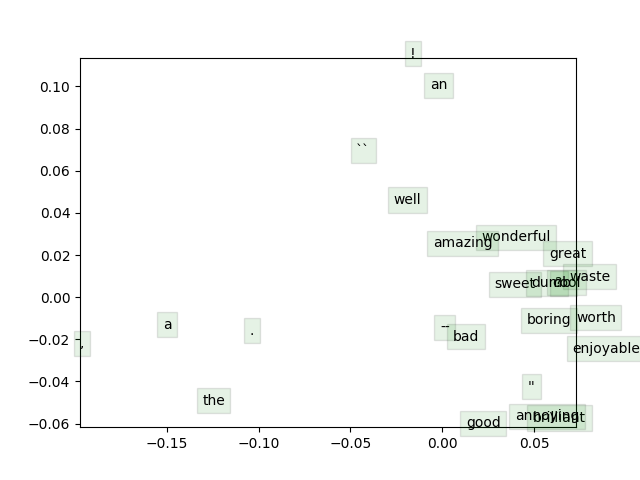
\includegraphics{assignment1/q3_word_vectors.png}

The plot is a 2-D projection of the word vectors trained from our corpus. We see that a number of generic quality-describing adjectives are clustered together (amazing, wonderful, great) along with some less general but still quite versatile ones (sweet, dumb, boring, enjoyable). Interestingly, ``waste" is also clustered pretty closely to these words; it is often used in a similar context (``x was a waste of time" vs. ``x was boring") although it is a noun rather than an adjective.
\end{document}
